\scanpage{259}
\begin{center}\uline{B O U R B A K I ' S\quad D I K T Ä T}\end{center}

Le prochain Congrès se tiendra du Lundi 25 juin au Samedi 7 juillet à Aiguines (Var), Auberge Relais, (tél. 9).

Pour les parisiens, départ le Dimanche 24 à 22 h 13, gare de Lyon, par le train autos-couchettes. Arrivée à Avignon à 7 h 23. Les voitures de Serre, Samuel, Bruhat emmèneront les voyageurs d'Avignon à Aiguines. Il est presque indispensable d'effectuer en même temps la location voiture et l'achat des billets aller et retour des voyageurs. Chacun est donc prié d'envoyer \uline{d'urgence} à Dixmier ses intentions précises concernant le voyage aller et le voyage retour.

Pour ceux qui n'utiliseront pas la méthode précédente, la moins mauvaise solution consiste à prendre le train jusqu'à Toulon, puis un car Toulon-Aups, puis un car Aups-Aiguines.

\uline{Programme} :

1) Algèbre commutative. Chap. VII, Diviseurs, § 4, Modules sur les anneaux intégralement clos, n° 353. (Apporter le n° 300, rapport d'Arithmétique. Samuel apportera une documentation).

2) La ramification dans les corps locaux (rédaction tirée en noir à Paris). Apporter le n° 363, (démonstration du théorème de Hasse-Arf).

3) ``Un bout de rédaction'' (il s'agit de la théorie de Morse). (Rédaction tirée en noir à Paris).

4) Algèbre, réédition du chap. III, n° 371, (Koszul apportera les épreuves de la réédition du chap. II).

Algèbres cayleyennes : n° 381.

5) Une rédaction sur les groupes de Lie qui doit être distribuée avant le Congrès. Apporter le n° 372 (Variétés de groupes ; groupes standard et applications) et le n° 340 (Variétés de groupes).

\margin{\figure{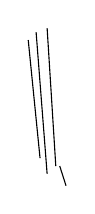
\begin{tikzpicture}[x=1cm,y=1cm]
\draw (0,1.7)--(.15,.2);\draw (.1,1.8)--(.24,0);\draw (.24,1.85)--(.35,.1);\draw (.4,.1)--(.48,-.15);
\end{tikzpicture}}}
6) Une rédaction sur les systèmes de racines qui doit être distribuée prochainement. Apporter le n° 351, et le papier de Tits (Groupes et géométries de Coxeter) tiré en noir à l'IHES.

7) Existence de représentations intégrales dans les convexes compacts : n° 379. Apporter le n° 378.

8) Algèbres normées, n° 380. Dixmier apportera une documentation.

\mspage{258}
